\section{\color{olive}Exercise 1: Tank Simulation}

\subsection{\color{purple}Moore's Finite State Machine}

Moore's Finite State Machine (FSM) follows a model where the next state of the machine is determined by the current
inputs and its current state, while the output is determined by the current state of the machine, following the
designed combinational logic.

\subsubsection{\color{orange}Design}

Given the specifications required of the pump controller, the functionality of the fsm was represented
on Figure \ref{fig:moore_flow} and on Table \ref{fig:moore_table}, where "LnA" stands for "Last not Activated".

\begin{figure}[H]
    \begin{center}
        \begin{tikzpicture}[node distance = 5cm, auto]
    %place nodes
    \node [block] (empty) {Empty B1:On B2:On};
    \node [decision, below of = empty] (toggle) {Last Not Activated Pump};
    \node [block, left of = toggle]  (only_one) {Half Full: B1:On B2:Off LnA=B2};
    \node [block, right of = toggle] (only_two) {Half Full: B1:Off B2:On LnA=B1};
    \node [block, below of = toggle] (full) {Full: B1:Off B2:Off};
    %place lines
    \path [line] (empty) -- node [near start] {I=1,S=0} (toggle);
    \path [line] (toggle) -- node [near start] {B1} (only_one);
    \path [line] (toggle) -- node [near start] {B2} (only_two);
    \path [line] (full) -- node [near start] {I=1,S=0} (toggle);
    \path [line] (only_one) |- node [near start] {I=1,S=1} (full);
    \path [line] (only_two) |- node [near start] {I=1,S=1} (full);
    \path [line] (only_one) |- node [near start] {I=0,S=0} (empty);
    \path [line] (only_two) |- node [near start] {I=0,S=0} (empty);

\end{tikzpicture}
        \caption{Flow Diagram for Moore's Machine}
        \label{fig:moore_flow}
    \end{center}
\end{figure}

\begin{table}[H]
    \begin{center}
        \begin{tabular}{|c|c|c|c|c|c|c|}
    \hline
    \multirow{3}{*}{Current State} & \multicolumn{4}{c}{Next State} & \multicolumn{2}{|c|}{Output} \\
    & S I & S I & S I & S I & \multirow{2}{*}{B1} & \multirow{2}{*}{B2} \\
    & 0 0 & 0 1 & 1 0 & 1 1 & & \\
    \hline
    Empty (0 0) & Empty & Half Full & Error & Full & 1 & 1 \\
    Half Full (0 1)& Empty & Half Full & Error & Full & $\sim$LnA & LnA \\
    Error (1 0)& Empty & Half Full & Error & Full & 0 & 0 \\
    Full (1 1)& Empty & Half Full & Error & Full & 0 & 0 \\
    \hline
\end{tabular}
        \caption{State Transition Table}
        \label{fig:moore_table}
    \end{center}
\end{table}

It can be observed that an error state was added. This was to cover every possible case of inputs. It was decided that
in case a "strange" input was received (Superior sensor activated while the Inferior sensor is not), both pumps should
stop working, as that seemed to be the safer decision, as this seemed to simply be a replenishment system and an empty
tank would alert the user of the error.

After deducing the combinational logic behind the next state assignment and the corresponding outputs for each state,
and taking into consideration the available components in the laboratory, the circuit in Figure \ref{fig:moore_circuit}
was obtained.

\begin{figure}[H]
    \begin{center}
        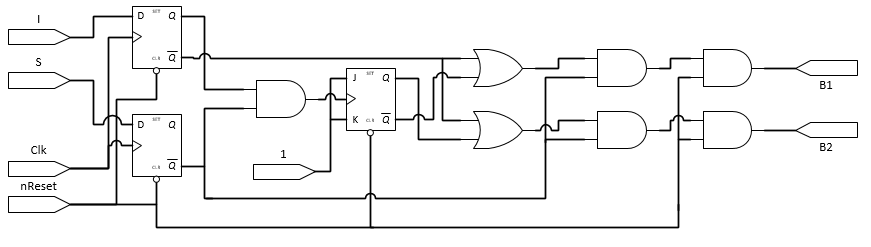
\includegraphics[width=\linewidth]{../Exercise1/Moore/report/circuit.png}
        \caption{Resulting circuit logic diagram}
        \label{fig:moore_circuit}
    \end{center}
\end{figure}

\subsubsection{\color{orange}Simulation}

Before physically implementing the FSM, first it was simulated in Verilog and ran through a testbench, 
where the waveform in Figure \ref{fig:moore_gtk} was obtained with gtkwave.

\begin{figure}[H]
    \begin{center}
        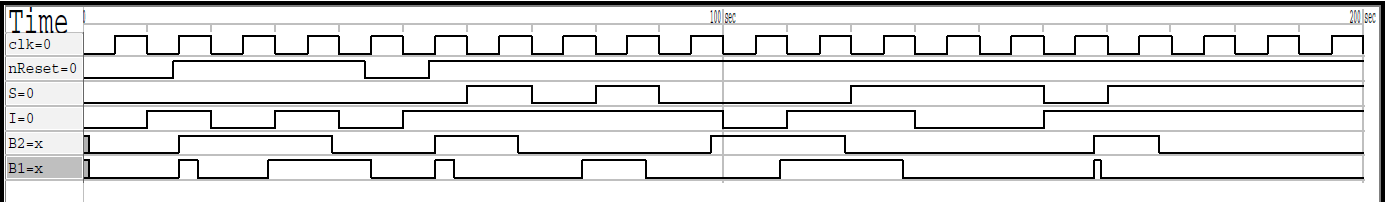
\includegraphics[width=\linewidth]{../Exercise1/Moore/report/gtkwave.png}
        \caption{Simulation results from gtkwave}
        \label{fig:moore_gtk}
    \end{center}
\end{figure}

It needs to be mentioned that in the design, a method of resetting the machine was included in case it was needed.
This reset case will set the LnA variable to 0 (which arms B1 for use) and deactivate both pumps until it is no longer
set.

\subsubsection{\color{orange}Physical Implementation}

After confirming the correct behaviour of the device, it was implemented on a Printed Circuit Board with the schematic
on Figure \ref{fig:moore_schem}.

\begin{figure}[H]
    \begin{center}
        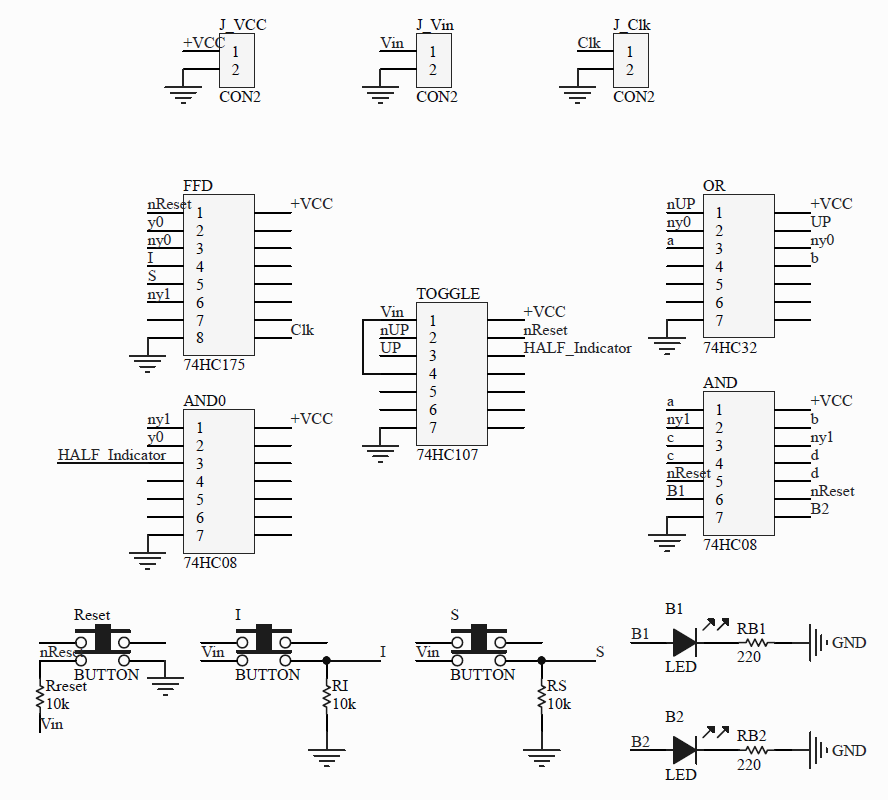
\includegraphics[scale=0.5]{../Exercise1/Moore/report/schematic.png}
        \caption{Device Schematic}
        \label{fig:moore_schem}
    \end{center}
\end{figure}

\begin{figure}[H]
    \begin{center}
        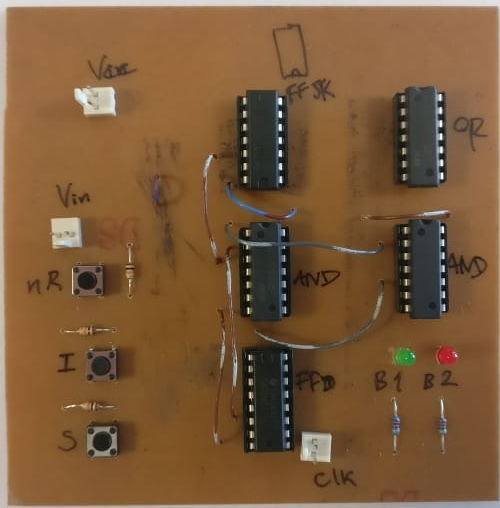
\includegraphics[scale=0.3]{../Exercise1/Moore/report/final_build.png}
        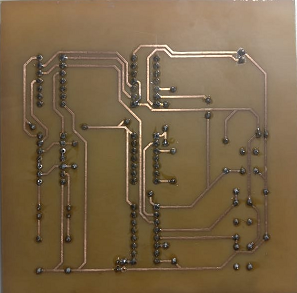
\includegraphics[scale=0.3]{../Exercise1/Moore/report/final_back.png}
        \caption{Final Physical device (front/back)}
        \label{fig:moore_build}
    \end{center}
\end{figure}

After it was fully implemented and tested, several measurements were taken to figure out its characteristics.
In Figures \ref{fig:moore_nres} and \ref{fig:moore_nres_delay} both the functionality and the delay between the output
and the reset input can be seen and were measured to be 6.6ns.

\begin{figure}[H]
    \begin{center}
        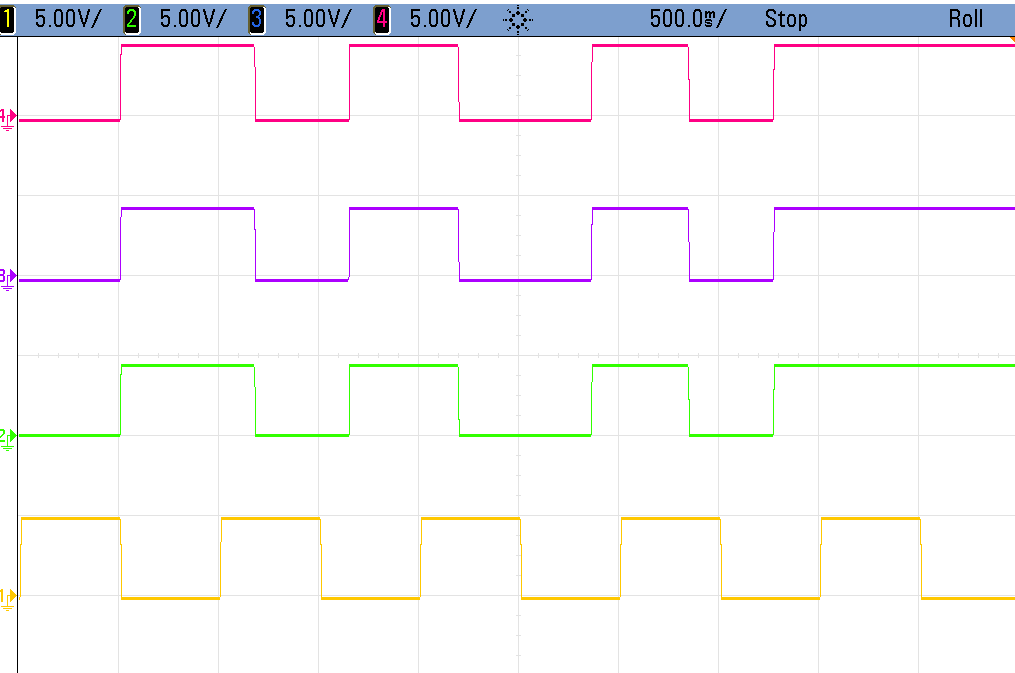
\includegraphics[scale=0.3]{../Exercise1/Moore/report/images/e3e1_1_4nreset.png}
        \caption{Reset (pink) functionality testing}
        \label{fig:moore_nres}
    \end{center}
\end{figure}

\begin{figure}[H]
    \begin{center}
        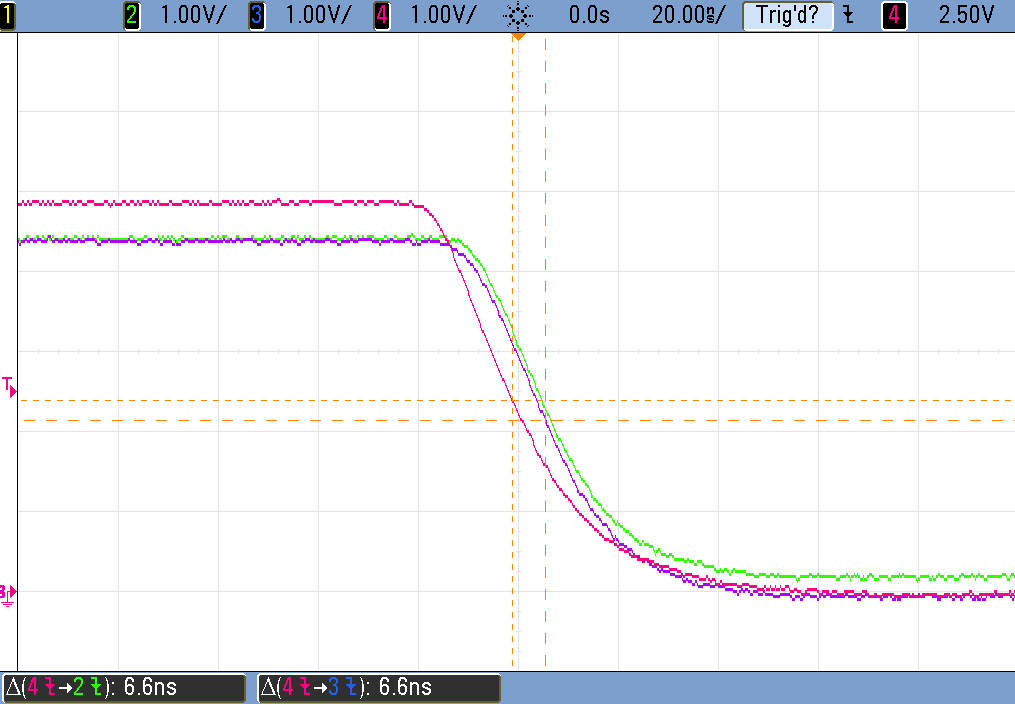
\includegraphics[scale=0.3]{../Exercise1/Moore/report/images/e3e1_nreset_delay.png}
        \caption{Reset (pink) delay measurements with B1(green) and B2(blue)}
        \label{fig:moore_nres_delay}
    \end{center}
\end{figure}

The delay between the clock's positive edge and the output signals was also measured to be around 30ns in Figure \ref{fig:moore_delays}.

\begin{figure}[H]
    \begin{center}
        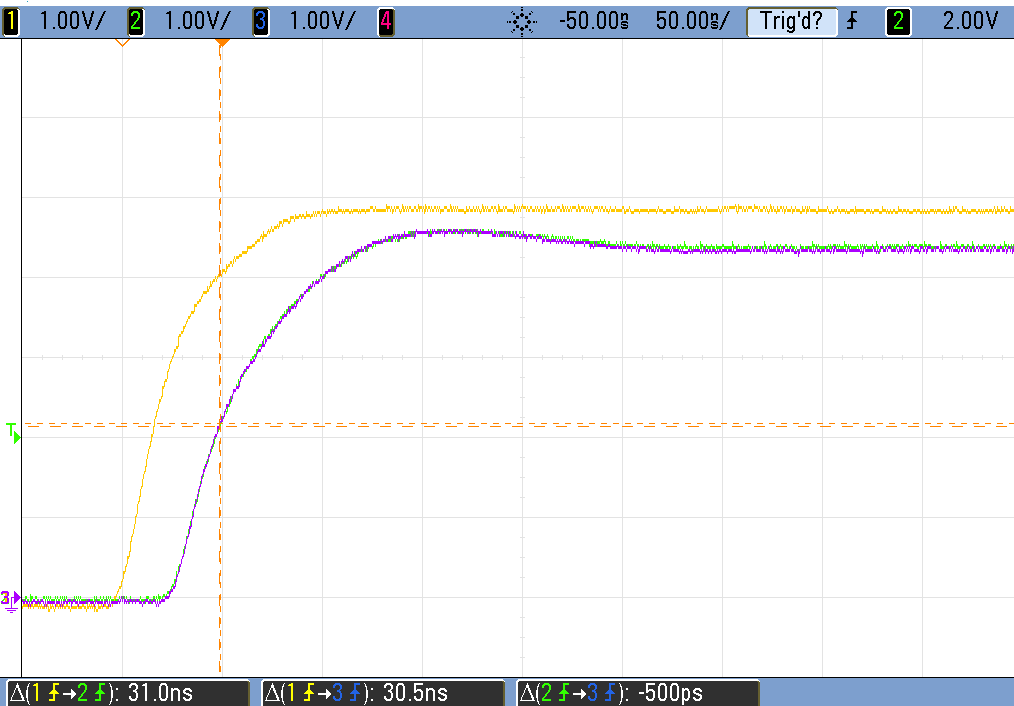
\includegraphics[scale=0.3]{../Exercise1/Moore/report/images/e3e1_1.png}\\
        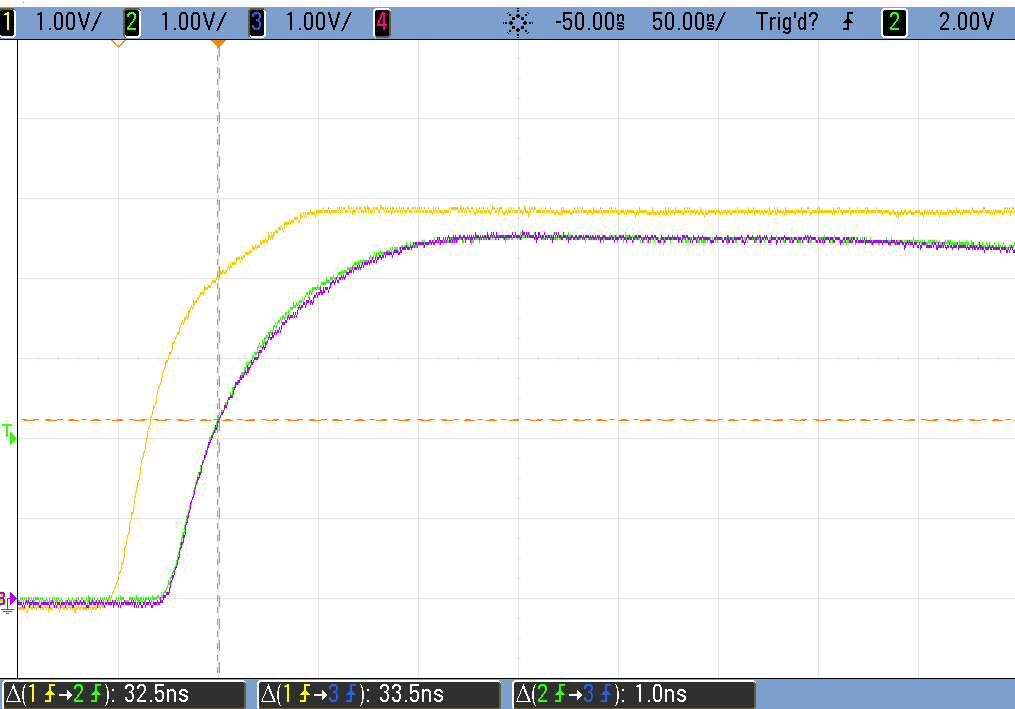
\includegraphics[scale=0.3]{../Exercise1/Moore/report/images/e3e1_1k.png}\\
        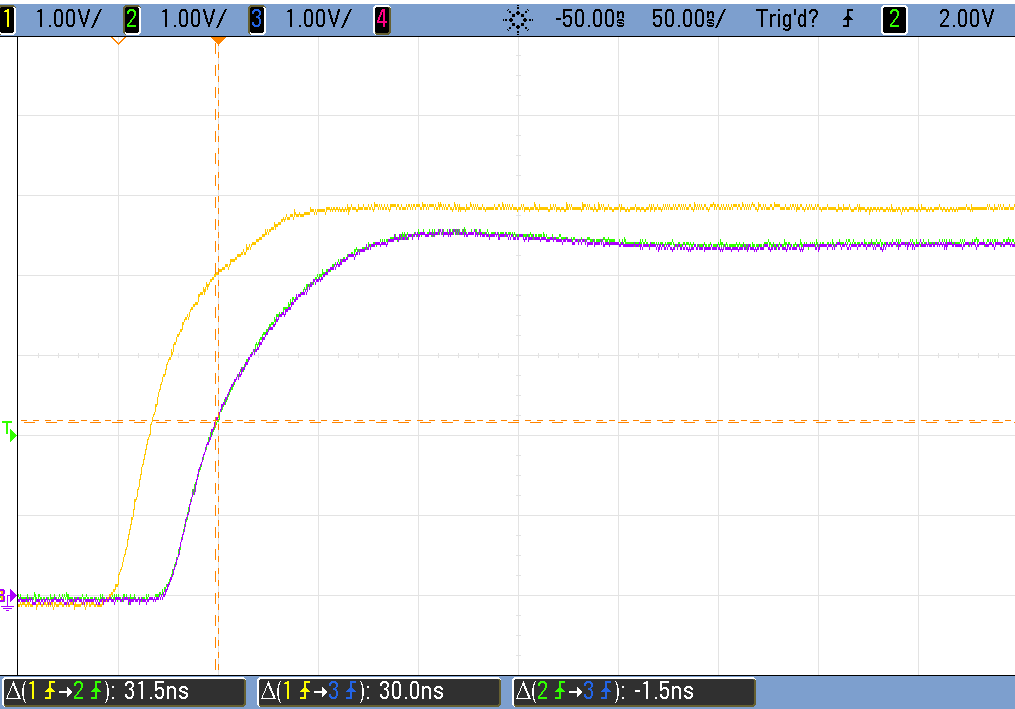
\includegraphics[scale=0.3]{../Exercise1/Moore/report/images/e3e1_100k_.png}
        \caption{I/O Delay measurements at 1Hz, 1 kHz and 100 kHz respectively}
        \label{fig:moore_delays}
    \end{center}
\end{figure}

Lastly, some general testing for the correct behaviour of the machine was tested, which was the one expected and
designed, as well as consistent to the one obtained in the Verilog simulation. From Figures \ref{fig:moore_max} and 
\ref{fig:moore_min} it can be seen that the maximum output voltage is around 4.3V when fed with a 5V source and a
minimum of near 0V, taking into account the noise.

\begin{figure}[H]
    \begin{center}
        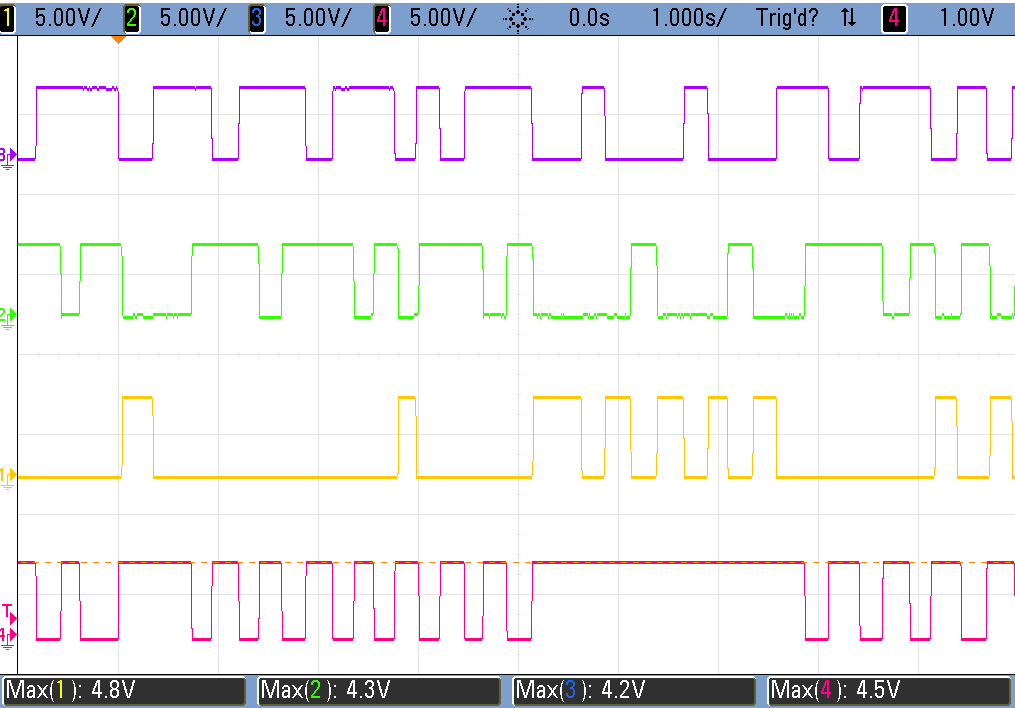
\includegraphics[scale=0.3]{../Exercise1/Moore/report/images/e3e1_1s4i_2b1_2b2_v1.png}
        \caption{High I/O voltage measurements}
        \label{fig:moore_max}
    \end{center}
\end{figure}

\begin{figure}[H]
    \begin{center}
        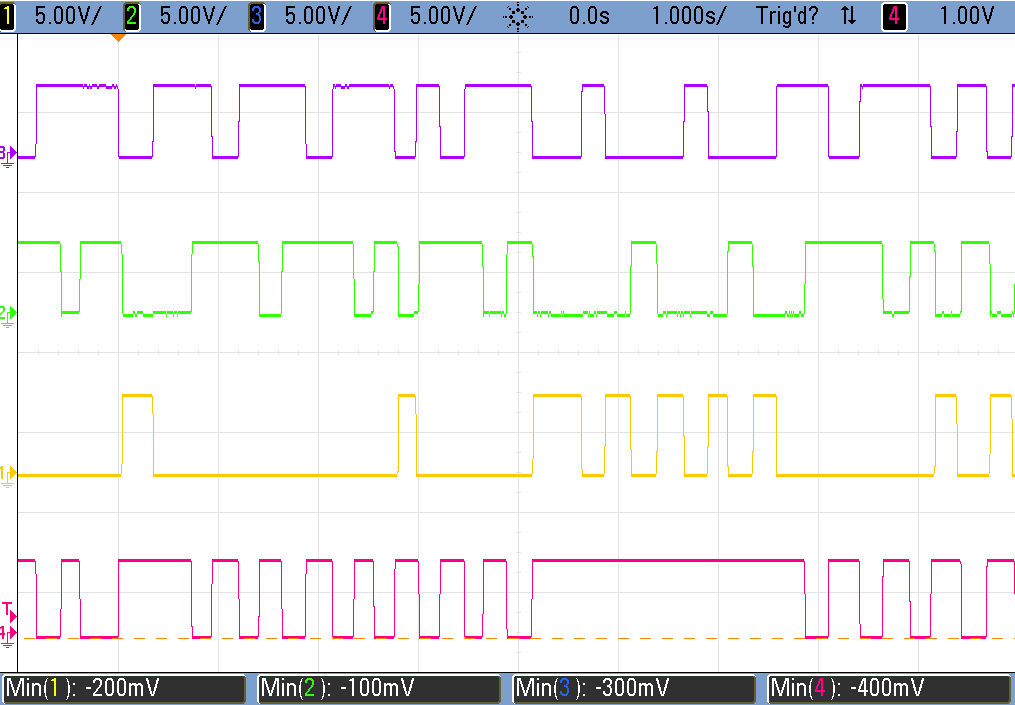
\includegraphics[scale=0.3]{../Exercise1/Moore/report/images/e3e1_1s4i_2b1_2b2_v0.png}
        \caption{Low I/O voltage measurements}
        \label{fig:moore_min}
    \end{center}
\end{figure}

\newpage
\subsubsection{\color{orange}Conclusions}
From all the measurements taken from the physical device and the simulations ran in Verilog, it can be concluded
that, given the case use this device would have, it is working as expected, with low delays between input and
output signals and accounting for all possible input cases, with a safety precausion of disabling all pumps from
activating if there is an error in the system or it is wished to be shut down.